%prescription_latex.tex

\documentclass{article}
\usepackage[utf8]{inputenc}
\usepackage[spanish]{babel}
\usepackage[T1]{fontenc}
\usepackage{textcomp}
\usepackage{graphicx}
\usepackage{eso-pic}
\usepackage{ifthen}
\usepackage[abs]{overpic}
\usepackage{pict2e,xcolor,varwidth}
\usepackage{color}
\usepackage{layout}
%\usepackage{tikz}
%\usepackage{relsize}
%\usepackage{etoolbox}
\usepackage[paperwidth=27.94cm, paperheight=21.59cm, left=0.0cm,right=0.0cm,top=0.0in,bottom=0.0in,headheight=0in,headsep=0pt,footskip=120pt]{geometry}
% Check parameters in: https://en.wikibooks.org/wiki/LaTeX/Page_Layout
%{# Define where latex finds images #}
{{ latex_graphics_path }}
%\setmainfont{Arial}
%\usepackage{fancyhdr}
%\usepackage{uarial}
%\usepackage[scaled]{uarial}
\usepackage{transparent}
%\usepackage[protrusion=true,expansion=true]{microtype}
%\usepackage{calc}
%\usepackage{verbatim}
%\makeatletter
%\g@addto@macro\@verbatim\small
%\makeatother 
\usepackage{xcolor}


\usepackage[export]{adjustbox}

%\usepackage{lmodern}
%\fontfamily{lmss}\selectfont
%\usepackage[utf8]{inputenc}
%\usepackage{unixode}


\begin{document}
\fontfamily{lmss}\selectfont
    % Include Background in ./prescript/media/media/template_v1.pdf
    % \AddToShipoutPictureBG{\ifthenelse{\isodd{\value{page}}}{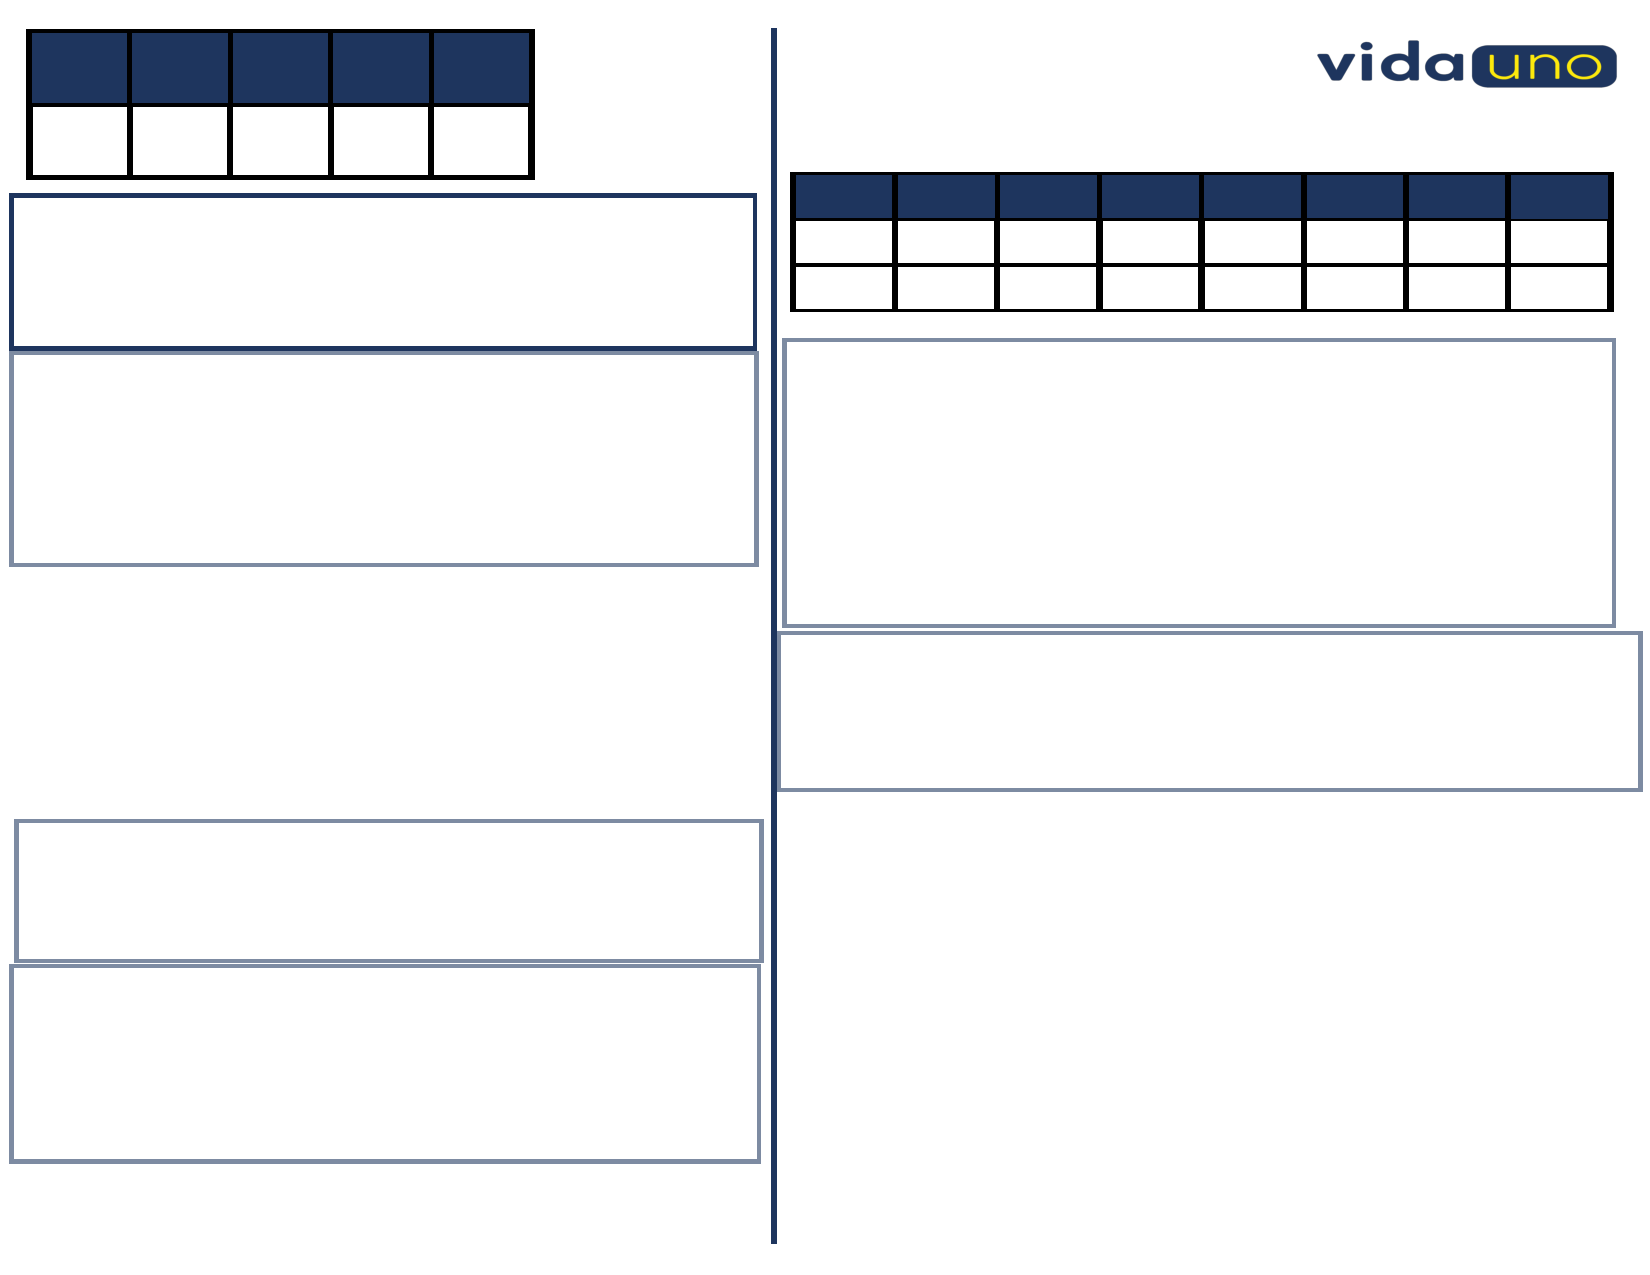
\includegraphics{laam_template}}{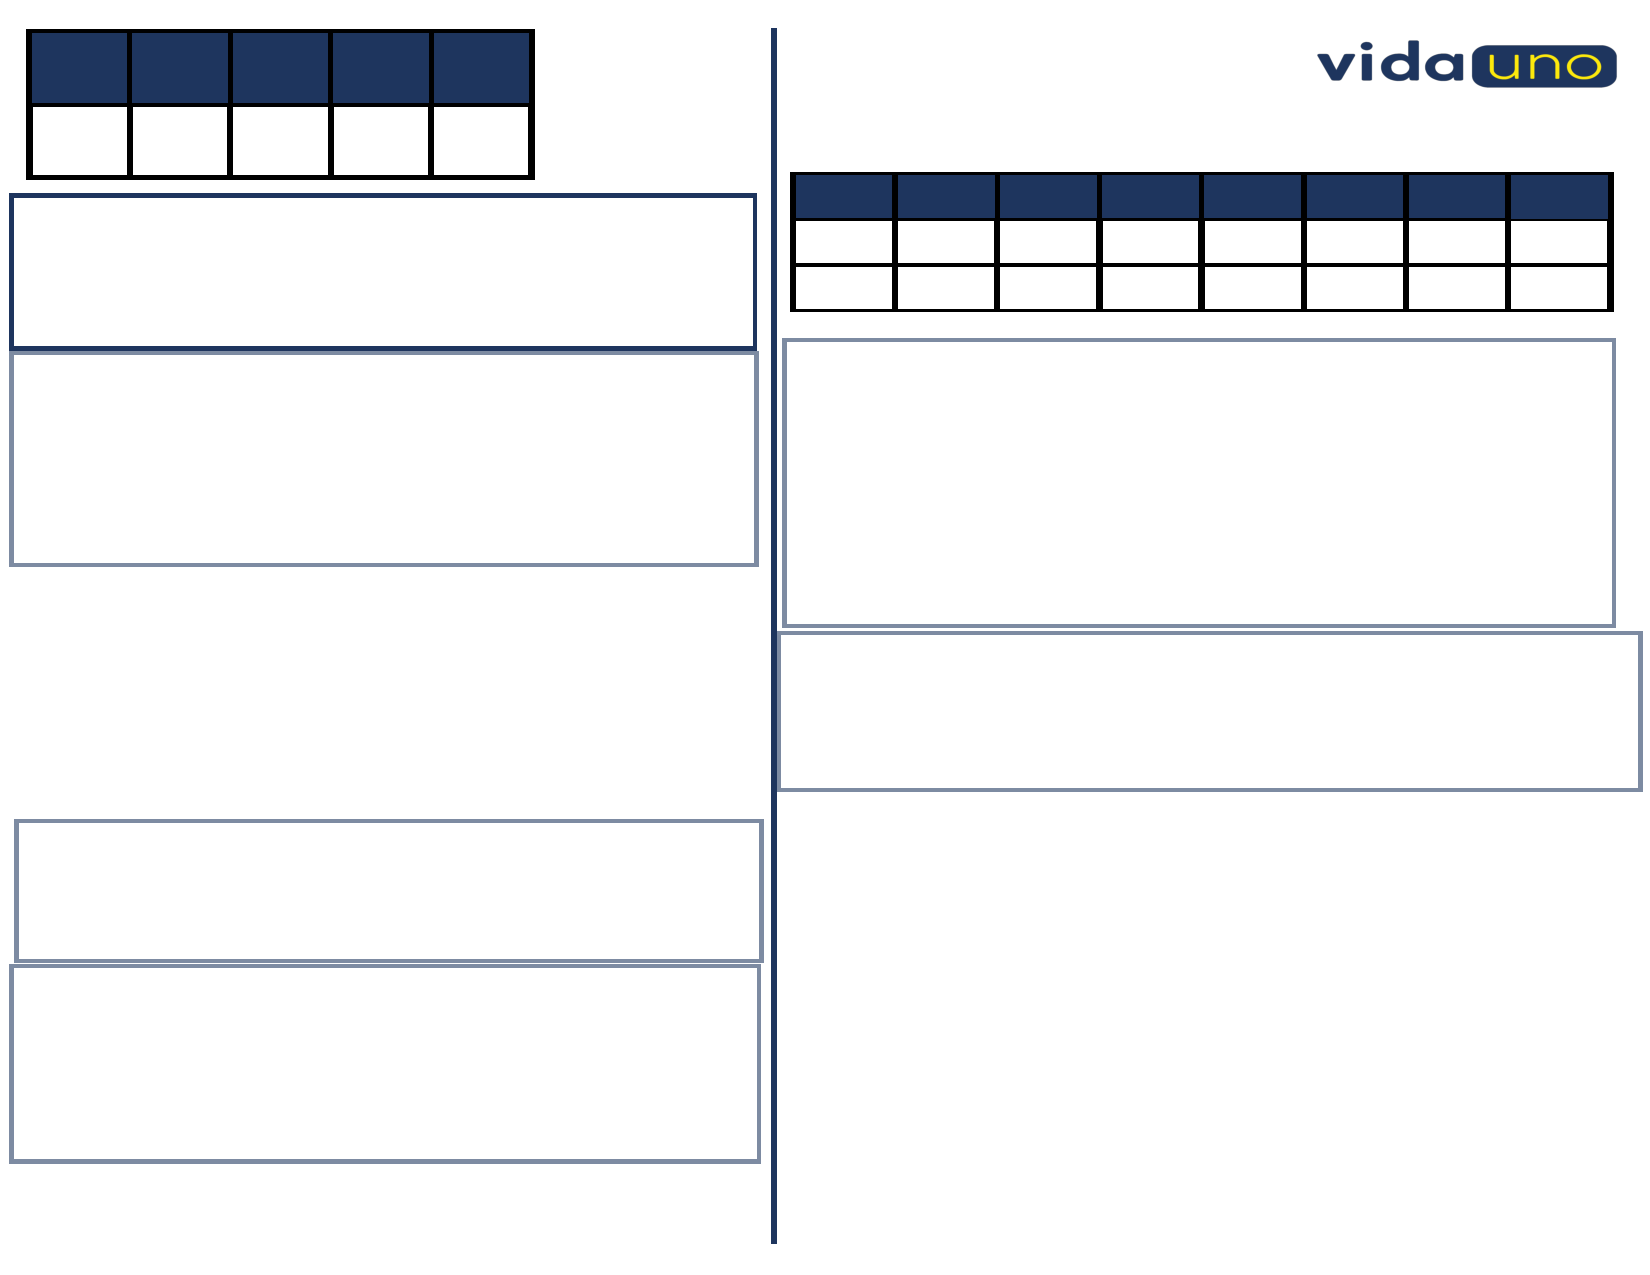
\includegraphics{laam_template}}}
    % Define page content
    %\textsf{\large{
    %\begin{changemargin}{1.5cm}{1.2cm}
        %\begin{enumerate}
            %{{ all_medications }}
            %bla!
        %\end{enumerate}
    %         \put(1,1){\parbox[t]{3cm}{\textsf{\large{
    %    \textbf{Consulta \#:} {{ content.id }}
    % }
    % }}}
        % Indicaciones Extra
        % \begin{enumerate}
        %     \textbf{Indicaciones Extra: \\ } {{ all_medications }}
        % \end{enumerate}
    %\end{changemargin}
    %}}
    % \begin{picture}(1,0.77272727)%
    %     %Consulta    
    % \put(200,0){\parbox[t]{3cm}{\textsf{\large{
    %    \textbf{{ content.id }}
    % }
    % }}}
    % \end{picture}
% \begingroup%
%   \makeatletter%
%   \providecommand\color[2][]{%
%     \errmessage{(Inkscape) Color is used for the text in Inkscape, but the package 'color.sty' is not loaded}%
%     \renewcommand\color[2][]{}%
%   }%
%   \providecommand\transparent[1]{%
%     \errmessage{(Inkscape) Transparency is used (non-zero) for the text in Inkscape, but the package 'transparent.sty' is not loaded}%
%     \renewcommand\transparent[1]{}%
%   }%
%   \providecommand\rotatebox[2]{#2}%
%   \newcommand\scaleInNode[1][1]{\tikzset{execute at begin node={\normalsize\larger[#1]}}}
%   \newcommand*\fsize{\dimexpr\f@size pt\relax}%
%   \newcommand*\lineheight[1]{\fontsize{\fsize}{#1\fsize}\selectfont}%
%   \ifx\svgwidth\undefined%
%     \setlength{\unitlength}{792bp}%
%     \ifx\svgscale\undefined%
%       \relax%
%     \else%
%       \setlength{\unitlength}{\unitlength * \real{\svgscale}}%
%     \fi%
%   \else%
%     \setlength{\unitlength}{\svgwidth}%
%   \fi%
%   \global\let\svgwidth\undefined%
%   \global\let\svgscale\undefined%
%   \makeatother%
%   \begin{picture}(1,0.77272727)%
%     \lineheight{1}%
%     \setlength\tabcolsep{0pt}%
%     \put(0,0){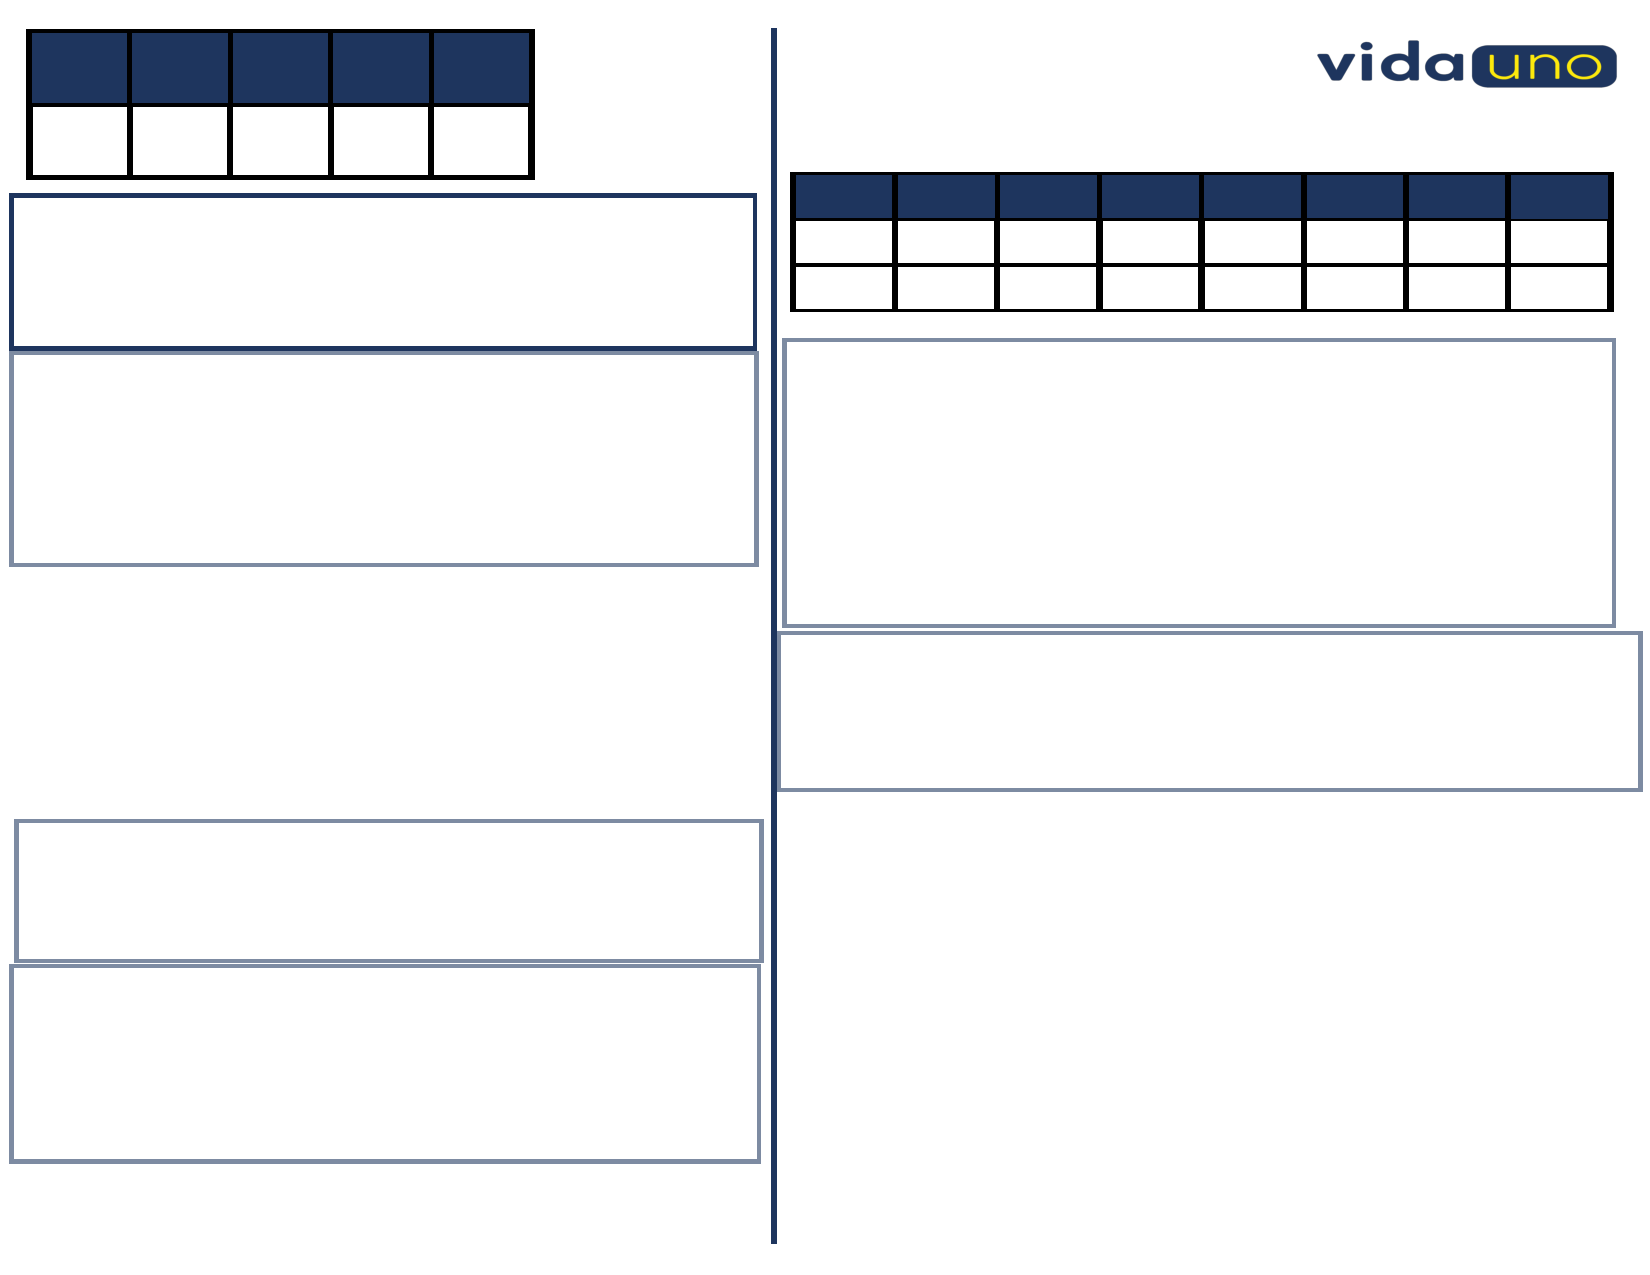
\includegraphics[width=\unitlength,page=1]{laam_template}}%

%     % \put(0.01140896,0.54355203){\parbox[t]{3cm}{\textsf{\large{
%     %    \textbf{Consulta \#:} {{ content.id }}
%     % }
%     % }}}
%     % \put(0.01140896,0.54355203){\color[rgb]{0.11764706,0.20784314,0.36862745}\makebox(0,0)[lt]{\lineheight{1.25}\smash{\begin{tabular}[t]{l}\textbf{Paciente desconocido {{content.id}} }\end{tabular}}}}%
% 	\put(0.42718184,0.73912713){\color[rgb]{0,0,0}\makebox(0,0)[lt]{\lineheight{1.25}\smash{\begin{tabular}[t]{l}\textit{ {{content.id}} }\end{tabular}}}}%
%    	\put(0.42718184,0.72336542){\color[rgb]{0,0,0}\makebox(0,0)[lt]{\lineheight{1.25}\smash{\begin{tabular}[t]{l}\textit{ {{content.service_unit }} }\end{tabular}}}}%
%     \put(0.3690564,0.69389968){\color[rgb]{0,0,0}\makebox(0,0)[lt]{\lineheight{1.25}\smash{\begin{tabular}[t]{l}\textit{ {{content.service_unit_type}} }\end{tabular}}}}%
%     \put(0.39254546,0.6775768){\color[rgb]{0,0,0}\makebox(0,0)[lt]{\lineheight{1.25}\smash{\begin{tabular}[t]{l}\textit{ {{content.service_unit_plate}} }\end{tabular}}}}%

%   \end{picture}%
% \endgroup%

\begin{figure}
  \centering
  \def\svgwidth{\columnwidth}
  %\input{paperless_template_6.pdf_tex}

\begingroup%
  \makeatletter%
  \providecommand\color[2][]{%
    \errmessage{(Inkscape) Color is used for the text in Inkscape, but the package 'color.sty' is not loaded}%
    \renewcommand\color[2][]{}%
  }%
  \providecommand\transparent[1]{%
    \errmessage{(Inkscape) Transparency is used (non-zero) for the text in Inkscape, but the package 'transparent.sty' is not loaded}%
    \renewcommand\transparent[1]{}%
  }%
  \providecommand\rotatebox[2]{#2}%
  \newcommand*\fsize{\dimexpr\f@size pt\relax}%
  \newcommand*\lineheight[1]{\fontsize{\fsize}{#1\fsize}\selectfont}%
  \ifx\svgwidth\undefined%
    \setlength{\unitlength}{782.27360219bp}%
    \ifx\svgscale\undefined%
      \relax%
    \else%
      \setlength{\unitlength}{\unitlength * \real{\svgscale}}%
    \fi%
  \else%
    \setlength{\unitlength}{\svgwidth}%
  \fi%
  \global\let\svgwidth\undefined%
  \global\let\svgscale\undefined%
  \makeatother%
  \begin{picture}(1,0.77245213)%
    \lineheight{1}%
    \setlength\tabcolsep{0pt}%
    \put(0,0){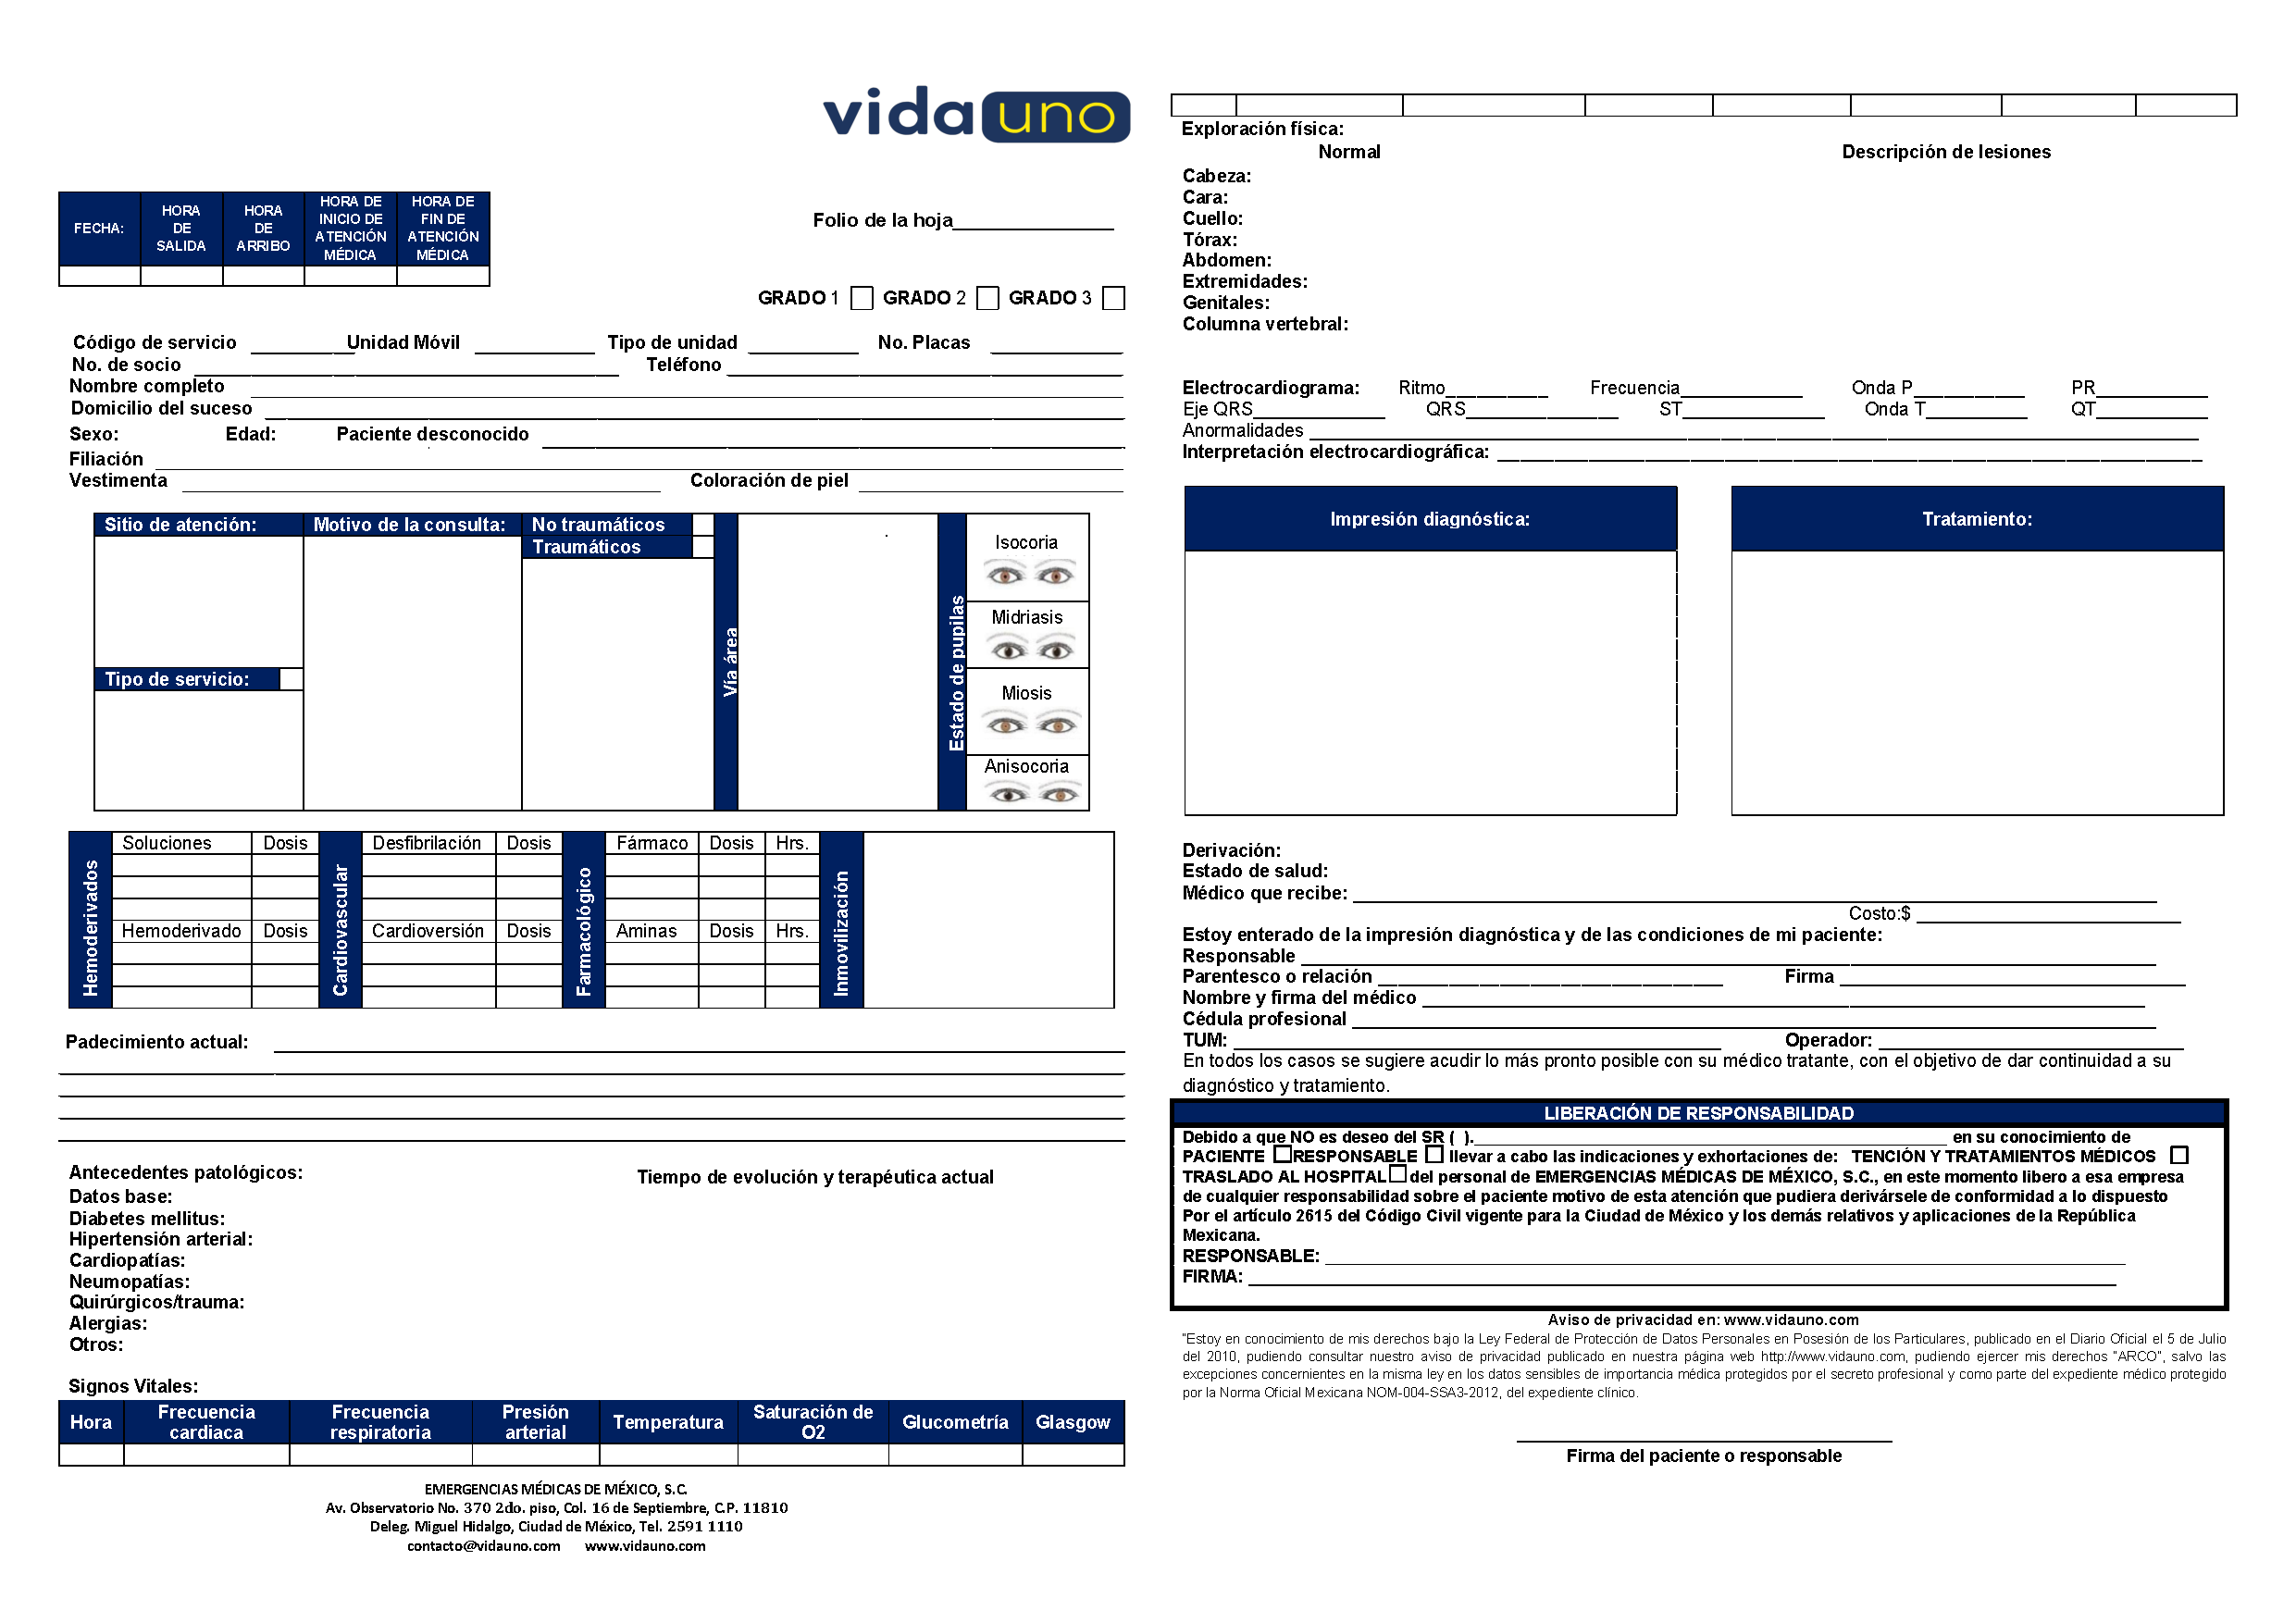
\includegraphics[width=\unitlength,page=1]{master_parte_medico}}%
    %\put(0.31336785,0.38838718){\includegraphics[scale=1]{test_image}}%
    %\put(0.78960956,0.24450476){
\includegraphics[scale=0.5]{client_signature}}%
    %Times
    \put(0.03117976,0.58432043){\color[rgb]{0.11764706,0.20784314,0.36862745}\makebox(0,0)[lt]{\lineheight{1.25}\smash{\begin{tabular}[t]{l}\fontfamily{lmss}\selectfont\tiny {{content.emergency_created_at}}\end{tabular}}}}%
    \put(0.06427789,0.58446308){\color[rgb]{0.11764706,0.20784314,0.36862745}\makebox(0,0)[lt]{\lineheight{1.25}\smash{\begin{tabular}[t]{l}\fontfamily{lmss}\selectfont\tiny {{content.unit_dispatched_time}}\end{tabular}}}}%
    \put(0.10029604,0.58387567){\color[rgb]{0.11764706,0.20784314,0.36862745}\makebox(0,0)[lt]{\lineheight{1.25}\smash{\begin{tabular}[t]{l}\fontfamily{lmss}\selectfont\tiny {{content.arrival_time}}\end{tabular}}}}%
    \put(0.13910523,0.58360406){\color[rgb]{0.11764706,0.20784314,0.36862745}\makebox(0,0)[lt]{\lineheight{1.25}\smash{\begin{tabular}[t]{l}\fontfamily{lmss}\selectfont\tiny {{content.attention_time}}\end{tabular}}}}%
    \put(0.17543913,0.58380438){\color[rgb]{0.11764706,0.20784314,0.36862745}\makebox(0,0)[lt]{\lineheight{1.25}\smash{\begin{tabular}[t]{l}\fontfamily{lmss}\selectfont\tiny {{content.final_emergency_time}}\end{tabular}}}}%

    
    \put(0.37115545,0.5742565){\color[rgb]{0.11764706,0.20784314,0.36862745}\makebox(0,0)[lt]{\lineheight{1.25}\smash{\begin{tabular}[t]{l}X\end{tabular}}}}%
    
    
    \put(0.42545332,0.57475133){\color[rgb]{0.11764706,0.20784314,0.36862745}\makebox(0,0)[lt]{\lineheight{1.25}\smash{\begin{tabular}[t]{l}X\end{tabular}}}}%
    
    
    \put(0.4811341,0.5742217){\color[rgb]{0.11764706,0.20784314,0.36862745}\makebox(0,0)[lt]{\lineheight{1.25}\smash{\begin{tabular}[t]{l}X\end{tabular}}}}%
    
    %Folio
    \put(0.41796551,0.60954148){\color[rgb]{0.11764706,0.20784314,0.36862745}\makebox(0,0)[lt]{\lineheight{1.25}\smash{\begin{tabular}[t]{l}\fontfamily{lmss}\selectfont\scriptsize {{content.id}}\end{tabular}}}}%

    \put(0.10902655,0.55515604){\color[rgb]{0.11764706,0.20784314,0.36862745}\makebox(0,0)[lt]{\lineheight{1.25}\smash{\begin{tabular}[t]{l}\fontfamily{lmss}\selectfont\scriptsize {{content.service_code}}\end{tabular}}}}%
    \put(0.20804855,0.55435574){\color[rgb]{0.11764706,0.20784314,0.36862745}\makebox(0,0)[lt]{\lineheight{1.25}\smash{\begin{tabular}[t]{l}\fontfamily{lmss}\selectfont\scriptsize {{content.service_unit}}\end{tabular}}}}%
   	\put(0.32826955,0.55435574){\color[rgb]{0.11764706,0.20784314,0.36862745}\makebox(0,0)[lt]{\lineheight{1.25}\smash{\begin{tabular}[t]{l}\fontfamily{lmss}\selectfont\scriptsize {{content.service_unit_type}}\end{tabular}}}}%
    \put(0.43247465,0.55435574){\color[rgb]{0.11764706,0.20784314,0.36862745}\makebox(0,0)[lt]{\lineheight{1.25}\smash{\begin{tabular}[t]{l}\fontfamily{lmss}\selectfont\scriptsize {{content.service_unit_plate}}\end{tabular}}}}%

    %Paciente
    \put(0.08748365,0.54597578){\color[rgb]{0.11764706,0.20784314,0.36862745}\makebox(0,0)[lt]{\lineheight{1.25}\smash{\begin{tabular}[t]{l}\fontfamily{lmss}\selectfont\scriptsize {{content.erste_code}} - {{content.odoo_client_name}}\end{tabular}}}}%
    \put(0.32347436,0.544854){\color[rgb]{0.11764706,0.20784314,0.36862745}\makebox(0,0)[lt]{\lineheight{1.25}\smash{\begin{tabular}[t]{l}\fontfamily{lmss}\selectfont\scriptsize {{content.patient_phone}}\end{tabular}}}}%
    \put(0.05306258,0.51467754){\color[rgb]{0.11764706,0.20784314,0.36862745}\makebox(0,0)[lt]{\lineheight{1.25}\smash{\begin{tabular}[t]{l}\fontfamily{lmss}\selectfont\scriptsize {{content.patient_gender}}\end{tabular}}}}%
    \put(0.12394486,0.51552412){\color[rgb]{0.11764706,0.20784314,0.36862745}\makebox(0,0)[lt]{\lineheight{1.25}\smash{\begin{tabular}[t]{l}\fontfamily{lmss}\selectfont\scriptsize {{content.patient_age}}\end{tabular}}}}%
    \put(0.11025071,0.53602224){\color[rgb]{0.11764706,0.20784314,0.36862745}\makebox(0,0)[lt]{\lineheight{1.25}\smash{\begin{tabular}[t]{l}\fontfamily{lmss}\selectfont\scriptsize {{content.patient_name}}\end{tabular}}}}%
    \put(0.11717691,0.52661865){\color[rgb]{0.11764706,0.20784314,0.36862745}\makebox(0,0)[lt]{\lineheight{1.25}\smash{\begin{tabular}[t]{l}\fontfamily{lmss}\selectfont\scriptsize {{content.patient_address}}\end{tabular}}}}%


    %Paciente desconocido
    \put(0.23723674,0.51552412){\color[rgb]{0.11764706,0.20784314,0.36862745}\makebox(0,0)[lt]{\lineheight{1.25}\smash{\begin{tabular}[t]{l}\fontfamily{lmss}\selectfont\scriptsize {{content.patient_unknow}}\end{tabular}}}}%
    \put(0.07146203,0.50540156){\color[rgb]{0.11764706,0.20784314,0.36862745}\makebox(0,0)[lt]{\lineheight{1.25}\smash{\begin{tabular}[t]{l}\fontfamily{lmss}\selectfont\scriptsize  {{content.patient_affiliations}}\end{tabular}}}}%
    \put(0.07920229,0.49404644){\color[rgb]{0.11764706,0.20784314,0.36862745}\makebox(0,0)[lt]{\lineheight{1.25}\smash{\begin{tabular}[t]{l}\fontfamily{lmss}\selectfont\scriptsize {{content.patient_clothes}}\end{tabular}}}}%
    \put(0.37437746,0.49499384){\color[rgb]{0.11764706,0.20784314,0.36862745}\makebox(0,0)[lt]{\lineheight{1.25}\smash{\begin{tabular}[t]{l}\fontfamily{lmss}\selectfont\scriptsize {{content.skin_color}}\end{tabular}}}}%

    %Padecimiento
    \put(0.11601621,0.2510955){\color[rgb]{0.11764706,0.20784314,0.36862745}\makebox(0,0)[lt]{\lineheight{1.25}\smash{\begin{tabular}[t]{l}\fontfamily{lmss}\selectfont\scriptsize {{content.fix_current_condition}}\end{tabular}}}}%
    %\put(0.02265882,0.24439213){\color[rgb]{0.11764706,0.20784314,0.36862745}\makebox(0,0)[lt]{\lineheight{1.25}\smash{\begin{tabular}[t]{l}\fontfamily{lmss}\selectfont {{content.current_condition}}\end{tabular}}}}%

    %Generales
    \put(0.04438815,0.46496172){\color[rgb]{0.11764706,0.20784314,0.36862745}\makebox(0,0)[lt]{\lineheight{1.25}\smash{\begin{tabular}[t]{l}\fontfamily{lmss}\selectfont\scriptsize {{content.attention_place}} \end{tabular}}}}%
    \put(0.04438815,0.39751941){\color[rgb]{0.11764706,0.20784314,0.36862745}\makebox(0,0)[lt]{\lineheight{1.25}\smash{\begin{tabular}[t]{l}\fontfamily{lmss}\selectfont\scriptsize {{content.service_type}} \end{tabular}}}}%
    
      \put(0.30180123,0.46556814){\color[rgb]{0.11764706,0.20784314,0.36862745}\makebox(0,0)[lt]{\lineheight{1.25}\smash{\begin{tabular}[t]{l}\fontfamily{lmss}\selectfont\scriptsize X \end{tabular}}}}%
    
      \put(0.3007691,0.47620579){\color[rgb]{0.11764706,0.20784314,0.36862745}\makebox(0,0)[lt]{\lineheight{1.25}\smash{\begin{tabular}[t]{l}\fontfamily{lmss}\selectfont\scriptsize X \end{tabular}}}}%
    
    %Trauma
    \put(0.23206628,0.45573384){\color[rgb]{0.11764706,0.20784314,0.36862745}\makebox(0,0)[lt]{\lineheight{0.8}\smash{\begin{tabular}[t]{l}\fontfamily{lmss}\selectfont\scriptsize {{ item }}\\\end{tabular}}}}%
    %Ojo Izquierdo
    %\put(0.20991809,0.36213786){\color[rgb]{0.11764706,0.20784314,0.36862745}\makebox(0,0)[lt]{\lineheight{1.25}\smash{\begin{tabular}[t]{l}\fontfamily{lmss}\selectfont Ojo Izquierdo: {{ item }},\end{tabular}}}}%
    %Ojo Derecho
    %\put(0.20991809,0.35077424){\color[rgb]{0.11764706,0.20784314,0.36862745}\makebox(0,0)[lt]{\lineheight{1.25}\smash{\begin{tabular}[t]{l}\fontfamily{lmss}\selectfont Ojo Derecho:  {{ item }},\end{tabular}}}}%
    \put(0.13358814,0.46425894){\color[rgb]{0.11764706,0.20784314,0.36862745}\makebox(0,0)[lt]{\lineheight{0.8}\smash{\begin{tabular}[t]{l}\fontfamily{lmss}\selectfont\scriptsize {{ item }}\\
    \end{tabular}}}}%
    %to_fix
    %Via Aerea
    \put(0.32505266,0.47551987){\color[rgb]{0.11764706,0.20784314,0.36862745}\makebox(0,0)[lt]{\lineheight{1.25}\smash{\begin{tabular}[t]{l}\fontfamily{lmss}\selectfont\scriptsize {{ item.airway_type}} - {{ item.instruction }}\\\end{tabular}}}}%

    
      
        \put(0.43392821,0.44715646){\color[rgb]{0.11764706,0.20784314,0.36862745}\makebox(0,0)[lt]{\lineheight{1.25}\smash{\begin{tabular}[t]{l}\textbf{X}\end{tabular}}}}%
      
      
        \put(0.43430823,0.41551969){\color[rgb]{0.11764706,0.20784314,0.36862745}\makebox(0,0)[lt]{\lineheight{1.25}\smash{\begin{tabular}[t]{l}\textbf{X}\end{tabular}}}}%
      
      
        \put(0.4335137,0.38189188){\color[rgb]{0.11764706,0.20784314,0.36862745}\makebox(0,0)[lt]{\lineheight{1.25}\smash{\begin{tabular}[t]{l}\textbf{X}\end{tabular}}}}%
      
          
        \put(0.43399571,0.35447078){\color[rgb]{0.11764706,0.20784314,0.36862745}\makebox(0,0)[lt]{\lineheight{1.25}\smash{\begin{tabular}[t]{l}\textbf{X}\end{tabular}}}}%
      
    
    
      
        \put(0.45563683,0.44651401){\color[rgb]{0.11764706,0.20784314,0.36862745}\makebox(0,0)[lt]{\lineheight{1.25}\smash{\begin{tabular}[t]{l}\textbf{X}\end{tabular}}}}%
      
      
        \put(0.45601685,0.41487724){\color[rgb]{0.11764706,0.20784314,0.36862745}\makebox(0,0)[lt]{\lineheight{1.25}\smash{\begin{tabular}[t]{l}\textbf{X}\end{tabular}}}}%
      
      
        \put(0.45522232,0.38124942){\color[rgb]{0.11764706,0.20784314,0.36862745}\makebox(0,0)[lt]{\lineheight{1.25}\smash{\begin{tabular}[t]{l}\textbf{X}\end{tabular}}}}%
      
        
        \put(0.45570433,0.35382833){\color[rgb]{0.11764706,0.20784314,0.36862745}\makebox(0,0)[lt]{\lineheight{1.25}\smash{\begin{tabular}[t]{l}\textbf{X}\end{tabular}}}}%
      
    



    %inmovilizacion
    \put(0.38134429,0.33628328){\color[rgb]{0.11764706,0.20784314,0.36862745}\makebox(0,0)[lt]{\lineheight{0.7}\smash{\begin{tabular}[t]{l}\fontfamily{lmss}\selectfont\scriptsize {{ item }}\\
    \end{tabular}}}}%

    %Impresion diagnostica
    \put(0.51738337,0.45891074){\color[rgb]{0.11764706,0.20784314,0.36862745}\makebox(0,0)[lt]{\lineheight{1.25}\smash{\begin{tabular}[t]{l}\fontfamily{lmss}\selectfont\scriptsize {{content.fix_diagnostic_impresion}}\end{tabular}}}}%
    %Tratamiento
    \put(0.75885924,0.45916877){\color[rgb]{0.11764706,0.20784314,0.36862745}\makebox(0,0)[lt]{\lineheight{1.25}\smash{\begin{tabular}[t]{l}\fontfamily{lmss}\selectfont\scriptsize {{content.fix_treatment}} \end{tabular}}}}%

    %Medicamentos (to_fix)
    %\put(0.0159714,0.27918911){\color[rgb]{0.11764706,0.20784314,0.36862745}\makebox(0,0)[lt]{\lineheight{1.25}\smash{\begin{tabular}[t]{l}\fontfamily{lmss}\selectfont {{ content.medications }}\end{tabular}}}}%
    %\put(0.0159714,0.27918911){\color[rgb]{0.11764706,0.20784314,0.36862745}\makebox(0,0)[lt]{\lineheight{1.25}\smash{\begin{tabular}[t]{l}\fontfamily{lmss}\selectfont la medi\end{tabular}}}}%
    %\put(0.0159714,0.27918911){\color[rgb]{0.11764706,0.20784314,0.36862745}\makebox(0,0)[lt]{\lineheight{1.25}\smash{\begin{tabular}[t]{l}\fontfamily{lmss}\selectfont {{ item.medication_type }} - {{ item.medication_name }} - {{ item.medication_hrs }} hrs\\\end{tabular}}}}%

    %Antecedentes
    %Diabetes
    %\put(0.48529688,0.5272494){\color[rgb]{0.11764706,0.20784314,0.36862745}\makebox(0,0)[lt]{\lineheight{1.25}\smash{\begin{tabular}[t]{l}\fontfamily{lmss}\selectfont Diabetes mellitus\end{tabular}}}}%
    \put(0.11758108,0.17376971){\color[rgb]{0.11764706,0.20784314,0.36862745}\makebox(0,0)[lt]{\lineheight{1.25}\smash{\begin{tabular}[t]{l}\fontfamily{lmss}\selectfont\scriptsize {{content.pathological_history_daibetes_melitus}}\end{tabular}}}}%
    \put(0.14099679,0.17376971){\color[rgb]{0.11764706,0.20784314,0.36862745}\makebox(0,0)[lt]{\lineheight{1.25}\smash{\begin{tabular}[t]{l}\fontfamily{lmss}\selectfont\scriptsize {{content.detail_pat_history_daibetes_melitus}}\end{tabular}}}}%

    % %Hipertension
    % \put(0.48529688,0.50503129){\color[rgb]{0.11764706,0.20784314,0.36862745}\makebox(0,0)[lt]{\lineheight{1.25}\smash{\begin{tabular}[t]{l}\fontfamily{lmss}\selectfont Hipertensión arterial:\end{tabular}}}}%
    \put(0.11758108,0.16393908){\color[rgb]{0.11764706,0.20784314,0.36862745}\makebox(0,0)[lt]{\lineheight{1.25}\smash{\begin{tabular}[t]{l}\fontfamily{lmss}\selectfont\scriptsize {{content.pathological_history_arterial_hypertension}}\end{tabular}}}}%
    \put(0.14099679,0.16393908){\color[rgb]{0.11764706,0.20784314,0.36862745}\makebox(0,0)[lt]{\lineheight{1.25}\smash{\begin{tabular}[t]{l}\fontfamily{lmss}\selectfont\scriptsize {{content.detail_pat_history_arterial_hypertension}}\end{tabular}}}}%

    % %Cardiopatias
    % \put(0.48529688,0.48172564){\color[rgb]{0.11764706,0.20784314,0.36862745}\makebox(0,0)[lt]{\lineheight{1.25}\smash{\begin{tabular}[t]{l}\fontfamily{lmss}\selectfont Cardiopatias \end{tabular}}}}%
    \put(0.11758108,0.15476708){\color[rgb]{0.11764706,0.20784314,0.36862745}\makebox(0,0)[lt]{\lineheight{1.25}\smash{\begin{tabular}[t]{l}\fontfamily{lmss}\selectfont\scriptsize {{content.pathological_history_heart_disease}} \end{tabular}}}}%   
    \put(0.14099679,0.15474248){\color[rgb]{0.11764706,0.20784314,0.36862745}\makebox(0,0)[lt]{\lineheight{1.25}\smash{\begin{tabular}[t]{l}\fontfamily{lmss}\selectfont\scriptsize {{content.detail_pat_history_heart_disease}} \end{tabular}}}}%
     
    % %Neumopatias
    % \put(0.48529688,0.45853652){\color[rgb]{0.11764706,0.20784314,0.36862745}\makebox(0,0)[lt]{\lineheight{1.25}\smash{\begin{tabular}[t]{l}\fontfamily{lmss}\selectfont Neumopatias\end{tabular}}}}%
    \put(0.11672491,0.14561334){\color[rgb]{0.11764706,0.20784314,0.36862745}\makebox(0,0)[lt]{\lineheight{1.25}\smash{\begin{tabular}[t]{l}\fontfamily{lmss}\selectfont\scriptsize {{content.pathological_history_pneumopathies}}\end{tabular}}}}%
    \put(0.14014062,0.14558873){\color[rgb]{0.11764706,0.20784314,0.36862745}\makebox(0,0)[lt]{\lineheight{1.25}\smash{\begin{tabular}[t]{l}\fontfamily{lmss}\selectfont\scriptsize {{content.detail_pat_history_pneumopathies}}\end{tabular}}}}%


    % %Trauma
    % \put(0.48715137,0.43527249){\color[rgb]{0.11764706,0.20784314,0.36862745}\makebox(0,0)[lt]{\lineheight{1.25}\smash{\begin{tabular}[t]{l}\fontfamily{lmss}\selectfont Quirurgicos/trauma:\end{tabular}}}}%
    \put(0.11758108,0.13647739){\color[rgb]{0.11764706,0.20784314,0.36862745}\makebox(0,0)[lt]{\lineheight{1.25}\smash{\begin{tabular}[t]{l}\fontfamily{lmss}\selectfont\scriptsize {{content.pathological_history_trauma}}\end{tabular}}}}%
    \put(0.14099679,0.13639128){\color[rgb]{0.11764706,0.20784314,0.36862745}\makebox(0,0)[lt]{\lineheight{1.25}\smash{\begin{tabular}[t]{l}\fontfamily{lmss}\selectfont\scriptsize {{content.detail_pat_history_trauma}}\end{tabular}}}}%


    % %Alergy
    % \put(0.48715137,0.41208615){\color[rgb]{0.11764706,0.20784314,0.36862745}\makebox(0,0)[lt]{\lineheight{1.25}\smash{\begin{tabular}[t]{l}\fontfamily{lmss}\selectfont Alergias\end{tabular}}}}%
    \put(0.11758108,0.12728379){\color[rgb]{0.11764706,0.20784314,0.36862745}\makebox(0,0)[lt]{\lineheight{1.25}\smash{\begin{tabular}[t]{l}\fontfamily{lmss}\selectfont\scriptsize {{content.pathological_history_alergy}}\end{tabular}}}}%
    \put(0.14099679,0.12719768){\color[rgb]{0.11764706,0.20784314,0.36862745}\makebox(0,0)[lt]{\lineheight{1.25}\smash{\begin{tabular}[t]{l}\fontfamily{lmss}\selectfont\scriptsize {{content.detail_pat_history_alergy}}\end{tabular}}}}%


    % %Other
    % \put(0.48715137,0.38762916){\color[rgb]{0.11764706,0.20784314,0.36862745}\makebox(0,0)[lt]{\lineheight{1.25}\smash{\begin{tabular}[t]{l}\fontfamily{lmss}\selectfont Otros\end{tabular}}}}%
    \put(0.11758108,0.11881088){\color[rgb]{0.11764706,0.20784314,0.36862745}\makebox(0,0)[lt]{\lineheight{1.25}\smash{\begin{tabular}[t]{l}\fontfamily{lmss}\selectfont\scriptsize {{content.other_pathological_history}}\end{tabular}}}}%
    %\put(0.59572153,0.38769855){\color[rgb]{0.11764706,0.20784314,0.36862745}\makebox(0,0)[lt]{\lineheight{1.25}\smash{\begin{tabular}[t]{l}\fontfamily{lmss}\selectfont No\end{tabular}}}}%    

    %Exploracion Fisica
    %Cabeza
    % \put(0.48349046,0.31358676){\color[rgb]{0.11764706,0.20784314,0.36862745}\makebox(0,0)[lt]{\lineheight{1.25}\smash{\begin{tabular}[t]{l}\fontfamily{lmss}\selectfont Cabeza\end{tabular}}}}%
    \put(0.5916532,0.62779907){\color[rgb]{0.11764706,0.20784314,0.36862745}\makebox(0,0)[lt]{\lineheight{1.25}\smash{\begin{tabular}[t]{l}\fontfamily{lmss}\selectfont\scriptsize {{content.normal_head}}\end{tabular}}}}%
    \put(0.61206298,0.62786673){\color[rgb]{0.11764706,0.20784314,0.36862745}\makebox(0,0)[lt]{\lineheight{1.25}\smash{\begin{tabular}[t]{l}\fontfamily{lmss}\selectfont\scriptsize {{content.det_normal_head}}\end{tabular}}}}%    
    % %Cara
    % \put(0.48349046,0.29763166){\color[rgb]{0.11764706,0.20784314,0.36862745}\makebox(0,0)[lt]{\lineheight{1.25}\smash{\begin{tabular}[t]{l}\fontfamily{lmss}\selectfont Cara\end{tabular}}}}%
    \put(0.5916532,0.6184675){\color[rgb]{0.11764706,0.20784314,0.36862745}\makebox(0,0)[lt]{\lineheight{1.25}\smash{\begin{tabular}[t]{l}\fontfamily{lmss}\selectfont\scriptsize {{content.normal_face}}\end{tabular}}}}%
    \put(0.61206298,0.61853516){\color[rgb]{0.11764706,0.20784314,0.36862745}\makebox(0,0)[lt]{\lineheight{1.25}\smash{\begin{tabular}[t]{l}\fontfamily{lmss}\selectfont\scriptsize {{content.det_normal_face}}\end{tabular}}}}%    
    % %Cuello
    % \put(0.48349046,0.28131895){\color[rgb]{0.11764706,0.20784314,0.36862745}\makebox(0,0)[lt]{\lineheight{1.25}\smash{\begin{tabular}[t]{l}\fontfamily{lmss}\selectfont Cuello\end{tabular}}}}%
    \put(0.5916532,0.60938371){\color[rgb]{0.11764706,0.20784314,0.36862745}\makebox(0,0)[lt]{\lineheight{1.25}\smash{\begin{tabular}[t]{l}\fontfamily{lmss}\selectfont\scriptsize {{content.normal_neck}}\end{tabular}}}}%
    \put(0.61206298,0.60956465){\color[rgb]{0.11764706,0.20784314,0.36862745}\makebox(0,0)[lt]{\lineheight{1.25}\smash{\begin{tabular}[t]{l}\fontfamily{lmss}\selectfont\scriptsize {{content.det_normal_neck}}\end{tabular}}}}%
    % %Torax
    % \put(0.48339183,0.26495693){\color[rgb]{0.11764706,0.20784314,0.36862745}\makebox(0,0)[lt]{\lineheight{1.25}\smash{\begin{tabular}[t]{l}\fontfamily{lmss}\selectfont Tórax\end{tabular}}}}%
    \put(0.5916532,0.6002403){\color[rgb]{0.11764706,0.20784314,0.36862745}\makebox(0,0)[lt]{\lineheight{1.25}\smash{\begin{tabular}[t]{l}\fontfamily{lmss}\selectfont\scriptsize {{content.normal_torax}}\end{tabular}}}}%
    \put(0.61206298,0.60042124){\color[rgb]{0.11764706,0.20784314,0.36862745}\makebox(0,0)[lt]{\lineheight{1.25}\smash{\begin{tabular}[t]{l}\fontfamily{lmss}\selectfont\scriptsize {{content.det_normal_torax}}\end{tabular}}}}%
    % %Abdomen
    % \put(0.48416864,0.24905109){\color[rgb]{0.11764706,0.20784314,0.36862745}\makebox(0,0)[lt]{\lineheight{1.25}\smash{\begin{tabular}[t]{l}\fontfamily{lmss}\selectfont Abdomen\end{tabular}}}}%
    \put(0.5916532,0.59110817){\color[rgb]{0.11764706,0.20784314,0.36862745}\makebox(0,0)[lt]{\lineheight{1.25}\smash{\begin{tabular}[t]{l}\fontfamily{lmss}\selectfont\scriptsize {{content.normal_abdomen}}\end{tabular}}}}%
    \put(0.61206298,0.59128911){\color[rgb]{0.11764706,0.20784314,0.36862745}\makebox(0,0)[lt]{\lineheight{1.25}\smash{\begin{tabular}[t]{l}\fontfamily{lmss}\selectfont\scriptsize {{content.det_normal_abdomen}}\end{tabular}}}}%
    % %Extremidades
    % \put(0.48373092,0.23278776){\color[rgb]{0.11764706,0.20784314,0.36862745}\makebox(0,0)[lt]{\lineheight{1.25}\smash{\begin{tabular}[t]{l}\fontfamily{lmss}\selectfont Extremidades\end{tabular}}}}%
    \put(0.5916532,0.58189295){\color[rgb]{0.11764706,0.20784314,0.36862745}\makebox(0,0)[lt]{\lineheight{1.25}\smash{\begin{tabular}[t]{l}\fontfamily{lmss}\selectfont\scriptsize {{content.normal_limbs}}\end{tabular}}}}%
    \put(0.61206298,0.58207389){\color[rgb]{0.11764706,0.20784314,0.36862745}\makebox(0,0)[lt]{\lineheight{1.25}\smash{\begin{tabular}[t]{l}\fontfamily{lmss}\selectfont\scriptsize {{content.det_normal_limbs}}\end{tabular}}}}%
    % %Genitales
    % \put(0.48348429,0.2166538){\color[rgb]{0.11764706,0.20784314,0.36862745}\makebox(0,0)[lt]{\lineheight{1.25}\smash{\begin{tabular}[t]{l}\fontfamily{lmss}\selectfont Genitales\end{tabular}}}}%
    \put(0.5916532,0.57279804){\color[rgb]{0.11764706,0.20784314,0.36862745}\makebox(0,0)[lt]{\lineheight{1.25}\smash{\begin{tabular}[t]{l}\fontfamily{lmss}\selectfont\scriptsize {{content.normal_genitals}}\end{tabular}}}}%
    \put(0.61206298,0.57297897){\color[rgb]{0.11764706,0.20784314,0.36862745}\makebox(0,0)[lt]{\lineheight{1.25}\smash{\begin{tabular}[t]{l}\fontfamily{lmss}\selectfont\scriptsize {{content.det_normal_genitals}}\end{tabular}}}}%
    % %Columna
    % \put(0.48349046,0.2025433){\color[rgb]{0.11764706,0.20784314,0.36862745}\makebox(0,0)[lt]{\lineheight{1.25}\smash{\begin{tabular}[t]{l}\fontfamily{lmss}\selectfont Columna \\Vertebral\end{tabular}}}}%
    \put(0.5916532,0.56347221){\color[rgb]{0.11764706,0.20784314,0.36862745}\makebox(0,0)[lt]{\lineheight{1.25}\smash{\begin{tabular}[t]{l}\fontfamily{lmss}\selectfont\scriptsize {{content.normal_spine}}\end{tabular}}}}%
    \put(0.61206298,0.56365314){\color[rgb]{0.11764706,0.20784314,0.36862745}\makebox(0,0)[lt]{\lineheight{1.25}\smash{\begin{tabular}[t]{l}\fontfamily{lmss}\selectfont\scriptsize {{content.det_normal_spine}}\end{tabular}}}}%
    %Electro
    \put(0.63149266,0.53664933){\color[rgb]{0.11764706,0.20784314,0.36862745}\makebox(0,0)[lt]{\lineheight{1.25}\smash{\begin{tabular}[t]{l}\fontfamily{lmss}\selectfont\scriptsize {{content.electro_rhythm}}\end{tabular}}}}%    
    \put(0.73355182,0.53601477){\color[rgb]{0.11764706,0.20784314,0.36862745}\makebox(0,0)[lt]{\lineheight{1.25}\smash{\begin{tabular}[t]{l}\fontfamily{lmss}\selectfont\scriptsize {{content.electro_frequency}}\end{tabular}}}}%
    \put(0.83566643,0.53611718){\color[rgb]{0.11764706,0.20784314,0.36862745}\makebox(0,0)[lt]{\lineheight{1.25}\smash{\begin{tabular}[t]{l}\fontfamily{lmss}\selectfont\scriptsize {{content.electro_wave_p}}\end{tabular}}}}%
    \put(0.91520486,0.53649172){\color[rgb]{0.11764706,0.20784314,0.36862745}\makebox(0,0)[lt]{\lineheight{1.25}\smash{\begin{tabular}[t]{l}\fontfamily{lmss}\selectfont\scriptsize {{content.electro_pr}}\end{tabular}}}}%
    \put(0.54866673,0.52688976){\color[rgb]{0.11764706,0.20784314,0.36862745}\makebox(0,0)[lt]{\lineheight{1.25}\smash{\begin{tabular}[t]{l}\fontfamily{lmss}\selectfont\scriptsize {{content.electro_axis_qrs}}\end{tabular}}}}%
    \put(0.64141646,0.52688976){\color[rgb]{0.11764706,0.20784314,0.36862745}\makebox(0,0)[lt]{\lineheight{1.25}\smash{\begin{tabular}[t]{l}\fontfamily{lmss}\selectfont\scriptsize {{content.electro_qrs}}\end{tabular}}}}%
    \put(0.73569805,0.52651523){\color[rgb]{0.11764706,0.20784314,0.36862745}\makebox(0,0)[lt]{\lineheight{1.25}\smash{\begin{tabular}[t]{l}\fontfamily{lmss}\selectfont\scriptsize {{content.electro_st}}\end{tabular}}}}%
    \put(0.84094359,0.52614065){\color[rgb]{0.11764706,0.20784314,0.36862745}\makebox(0,0)[lt]{\lineheight{1.25}\smash{\begin{tabular}[t]{l}\fontfamily{lmss}\selectfont\scriptsize {{content.electro_wave_t}}\end{tabular}}}}%
    \put(0.91520486,0.52665127){\color[rgb]{0.11764706,0.20784314,0.36862745}\makebox(0,0)[lt]{\lineheight{1.25}\smash{\begin{tabular}[t]{l}\fontfamily{lmss}\selectfont\scriptsize {{content.electro_qt}}\end{tabular}}}}%    
    \put(0.56987944,0.51728776){\color[rgb]{0.11764706,0.20784314,0.36862745}\makebox(0,0)[lt]{\lineheight{1.25}\smash{\begin{tabular}[t]{l}\fontfamily{lmss}\selectfont\scriptsize {{content.electro_abnormalities}}\end{tabular}}}}%
    \put(0.65016698,0.50867338){\color[rgb]{0.11764706,0.20784314,0.36862745}\makebox(0,0)[lt]{\lineheight{1.25}\smash{\begin{tabular}[t]{l}\fontfamily{lmss}\selectfont\scriptsize {{content.electro_interpretation}}\end{tabular}}}}%
    %Signos Vitales 1
    
    \put(0.0271255,0.07062683){\color[rgb]{0.11764706,0.20784314,0.36862745}\makebox(0,0)[lt]{\lineheight{1.25}\smash{\begin{tabular}[t]{l}\fontfamily{lmss}\selectfont\tiny {{ item.time|slice:"11:" }} \end{tabular}}}}%
    \put(0.05802029,0.07053194){\color[rgb]{0.11764706,0.20784314,0.36862745}\makebox(0,0)[lt]{\lineheight{1.25}\smash{\begin{tabular}[t]{l}\fontfamily{lmss}\selectfont\tiny {{ item.heart_rate }}\end{tabular}}}}%
    \put(0.13098371,0.07106162){\color[rgb]{0.11764706,0.20784314,0.36862745}\makebox(0,0)[lt]{\lineheight{1.25}\smash{\begin{tabular}[t]{l}\fontfamily{lmss}\selectfont\tiny {{ item.respiratory_rate}}\end{tabular}}}}%
    \put(0.20988188,0.07106162){\color[rgb]{0.11764706,0.20784314,0.36862745}\makebox(0,0)[lt]{\lineheight{1.25}\smash{\begin{tabular}[t]{l}\fontfamily{lmss}\selectfont\tiny {{ item.blood_pressure}}\end{tabular}}}}%
    \put(0.26601422,0.07073227){\color[rgb]{0.11764706,0.20784314,0.36862745}\makebox(0,0)[lt]{\lineheight{1.25}\smash{\begin{tabular}[t]{l}\fontfamily{lmss}\selectfont\tiny {{ item.temperature}}\end{tabular}}}}%
    \put(0.32533826,0.07106162){\color[rgb]{0.11764706,0.20784314,0.36862745}\makebox(0,0)[lt]{\lineheight{1.25}\smash{\begin{tabular}[t]{l}\fontfamily{lmss}\selectfont\tiny {{ item.oxygen_saturation}}\end{tabular}}}}%
    \put(0.39526948,0.07106162){\color[rgb]{0.11764706,0.20784314,0.36862745}\makebox(0,0)[lt]{\lineheight{1.25}\smash{\begin{tabular}[t]{l}\fontfamily{lmss}\selectfont\tiny {{ item.glucometry}}\end{tabular}}}}%
    \put(0.4490251,0.07053194){\color[rgb]{0.11764706,0.20784314,0.36862745}\makebox(0,0)[lt]{\lineheight{1.25}\smash{\begin{tabular}[t]{l}\fontfamily{lmss}\selectfont\tiny {{ item.glassgow_total }}\end{tabular}}}}%
    
    %Signos Vitales 2
    %\put(0.48899072,0.59441199){\color[rgb]{0.11764706,0.20784314,0.36862745}\makebox(0,0)[lt]{\lineheight{1.25}\smash{\begin{tabular}[t]{l}\fontfamily{lmss}\selectfont 12:41\end{tabular}}}}%
    %\put(0.56346295,0.59441199){\color[rgb]{0.11764706,0.20784314,0.36862745}\makebox(0,0)[lt]{\lineheight{1.25}\smash{\begin{tabular}[t]{l}\fontfamily{lmss}\selectfont 220\end{tabular}}}}%
    %\put(0.62325414,0.59432876){\color[rgb]{0.11764706,0.20784314,0.36862745}\makebox(0,0)[lt]{\lineheight{1.25}\smash{\begin{tabular}[t]{l}\fontfamily{lmss}\selectfont 321\end{tabular}}}}%
    %\put(0.68836013,0.59432876){\color[rgb]{0.11764706,0.20784314,0.36862745}\makebox(0,0)[lt]{\lineheight{1.25}\smash{\begin{tabular}[t]{l}\fontfamily{lmss}\selectfont 422\end{tabular}}}}%
    %\put(0.74651878,0.59441199){\color[rgb]{0.11764706,0.20784314,0.36862745}\makebox(0,0)[lt]{\lineheight{1.25}\smash{\begin{tabular}[t]{l}\fontfamily{lmss}\selectfont 523\end{tabular}}}}%
    %\put(0.81241818,0.59432876){\color[rgb]{0.11764706,0.20784314,0.36862745}\makebox(0,0)[lt]{\lineheight{1.25}\smash{\begin{tabular}[t]{l}\fontfamily{lmss}\selectfont 624\end{tabular}}}}%
    %\put(0.87214411,0.59441199){\color[rgb]{0.11764706,0.20784314,0.36862745}\makebox(0,0)[lt]{\lineheight{1.25}\smash{\begin{tabular}[t]{l}\fontfamily{lmss}\selectfont 725\end{tabular}}}}%
    %\put(0.93275252,0.59441199){\color[rgb]{0.11764706,0.20784314,0.36862745}\makebox(0,0)[lt]{\lineheight{1.25}\smash{\begin{tabular}[t]{l}\fontfamily{lmss}\selectfont 826\end{tabular}}}}%

    %Derivacion
    \put(0.56632851,0.33413518){\color[rgb]{0.11764706,0.20784314,0.36862745}\makebox(0,0)[lt]{\lineheight{1.25}\smash{\begin{tabular}[t]{l}\fontfamily{lmss}\selectfont\scriptsize {{content.derivation_type}} - {{content.derivation_hospital}}\end{tabular}}}}%
    %\put(0.56751227,0.6721787){\color[rgb]{0.11764706,0.20784314,0.36862745}\makebox(0,0)[lt]{\lineheight{1.25}\smash{\begin{tabular}[t]{l}\fontfamily{lmss}\selectfont {{content.derivation_hospital}}\end{tabular}}}}%
    \put(0.59086359,0.32494157){\color[rgb]{0.11764706,0.20784314,0.36862745}\makebox(0,0)[lt]{\lineheight{1.25}\smash{\begin{tabular}[t]{l}\fontfamily{lmss}\selectfont\scriptsize {{content.state_of_health}}\end{tabular}}}}%
    \put(0.5890775,0.31621801){\color[rgb]{0.11764706,0.20784314,0.36862745}\makebox(0,0)[lt]{\lineheight{1.25}\smash{\begin{tabular}[t]{l}\fontfamily{lmss}\selectfont\scriptsize {{content.derivation_recive}}\end{tabular}}}}%    
    \put(0.83680772,0.30734249){\color[rgb]{0.11764706,0.20784314,0.36862745}\makebox(0,0)[lt]{\lineheight{1.25}\smash{\begin{tabular}[t]{l}\fontfamily{lmss}\selectfont\scriptsize {{content.derivation_amount}}\end{tabular}}}}%

    %Finalizacion
    \put(0.56613143,0.28790386){\color[rgb]{0.11764706,0.20784314,0.36862745}\makebox(0,0)[lt]{\lineheight{1.25}\smash{\begin{tabular}[t]{l}\fontfamily{lmss}\selectfont\scriptsize {{content.demarcation_responsable}}\end{tabular}}}}%\
    \put(0.59939617,0.27975509){\color[rgb]{0.11764706,0.20784314,0.36862745}\makebox(0,0)[lt]{\lineheight{1.25}\smash{\begin{tabular}[t]{l}\fontfamily{lmss}\selectfont\scriptsize {{content.demarcation_relation}}\end{tabular}}}}%
    \put(0.61896758,0.26988471){\color[rgb]{0.11764706,0.20784314,0.36862745}\makebox(0,0)[lt]{\lineheight{1.25}\smash{\begin{tabular}[t]{l}\fontfamily{lmss}\selectfont\scriptsize {{content.crew_medic}}\end{tabular}}}}%
    \put(0.59042647,0.26068666){\color[rgb]{0.11764706,0.20784314,0.36862745}\makebox(0,0)[lt]{\lineheight{1.25}\smash{\begin{tabular}[t]{l}\fontfamily{lmss}\selectfont\scriptsize {{content.crew_medic_id_card}}\end{tabular}}}}%
    \put(0.53599859,0.25148177){\color[rgb]{0.11764706,0.20784314,0.36862745}\makebox(0,0)[lt]{\lineheight{1.25}\smash{\begin{tabular}[t]{l}\fontfamily{lmss}\selectfont\scriptsize {{content.crew_tum}}\end{tabular}}}}%
    \put(0.81652804,0.25194696){\color[rgb]{0.11764706,0.20784314,0.36862745}\makebox(0,0)[lt]{\lineheight{1.25}\smash{\begin{tabular}[t]{l}\fontfamily{lmss}\selectfont\scriptsize {{content.crew_operator}}\end{tabular}}}}%

    
      \put(0.79939617,0.25975509){
\includegraphics[scale=0.3]{signature_medic}}%
      %\put(0.78960956,0.44450476){\color[rgb]{0.11764706,0.20784314,0.36862745}\makebox(0,0)[lt]{\lineheight{1.25}\smash{\begin{tabular}[t]{l}\fontfamily{lmss}\selectfont Firma Médico\end{tabular}}}}%
    

    
    \put(0.58960956,0.11450476){
\includegraphics[scale=0.5]{client_signature}}%
    \put(0.64203741,0.04450476){
\includegraphics[scale=0.5]{client_signature}}%
    %\put((0.64203741,0.06450476){
\includegraphics[scale=0.5]{client_signature}}%
    \put(.64090291,0.20857036){\color[rgb]{0.11764706,0.20784314,0.36862745}\makebox(0,0)[lt]{\lineheight{1.25}\smash{\begin{tabular}[t]{l}\fontfamily{lmss}\selectfont\scriptsize {{content.demarcation_responsable}}\end{tabular}}}}%
    %\put(0.64203741,0.06450476){\color[rgb]{0.11764706,0.20784314,0.36862745}\makebox(0,0)[lt]{\lineheight{1.25}\smash{\begin{tabular}[t]{l}\fontfamily{lmss}\selectfont {{content.demarcation_responsable}}\end{tabular}}}}%
    

  \end{picture}
\endgroup%
\end{figure}

% \newpage

% \begin{figure}
%   \centering
%   \def\svgwidth{\columnwidth}
%   %\input{paperless_template_6.pdf_tex}

% \begingroup%
%   \makeatletter%
%   \providecommand\color[2][]{%
%     \errmessage{(Inkscape) Color is used for the text in Inkscape, but the package 'color.sty' is not loaded}%
%     \renewcommand\color[2][]{}%
%   }%
%   \providecommand\transparent[1]{%
%     \errmessage{(Inkscape) Transparency is used (non-zero) for the text in Inkscape, but the package 'transparent.sty' is not loaded}%
%     \renewcommand\transparent[1]{}%
%   }%
%   \providecommand\rotatebox[2]{#2}%
%   \newcommand*\fsize{\dimexpr\f@size pt\relax}%
%   \newcommand*\lineheight[1]{\fontsize{\fsize}{#1\fsize}\selectfont}%
%   \ifx\svgwidth\undefined%
%     \setlength{\unitlength}{782.27360219bp}%
%     \ifx\svgscale\undefined%
%       \relax%
%     \else%
%       \setlength{\unitlength}{\unitlength * \real{\svgscale}}%
%     \fi%
%   \else%
%     \setlength{\unitlength}{\svgwidth}%
%   \fi%
%   \global\let\svgwidth\undefined%
%   \global\let\svgscale\undefined%
%   \makeatother%
%   \begin{picture}(1,0.77245213)%
%     \lineheight{1}%
%     \setlength\tabcolsep{0pt}%
%     \put(0,0){\includegraphics[width=\unitlength,page=1]{parte_medico_master}}%
%     
%     \put(0.78960956,0.18450476){
\includegraphics[scale=0.5]{client_signature}}%
%     \put(0.64203741,0.01450476){
\includegraphics[scale=0.5]{client_signature}}%
%     %\put((0.64203741,0.06450476){
\includegraphics[scale=0.5]{client_signature}}%
%     \put(0.64203741,0.20450476){\color[rgb]{0.11764706,0.20784314,0.36862745}\makebox(0,0)[lt]{\lineheight{1.25}\smash{\begin{tabular}[t]{l}\fontfamily{lmss}\selectfont {{content.demarcation_responsable}}\end{tabular}}}}%
%     %\put(0.64203741,0.06450476){\color[rgb]{0.11764706,0.20784314,0.36862745}\makebox(0,0)[lt]{\lineheight{1.25}\smash{\begin{tabular}[t]{l}\fontfamily{lmss}\selectfont {{content.demarcation_responsable}}\end{tabular}}}}%
%     
%     
%     \put(0.78960956,0.46450476){
\includegraphics[scale=0.5,frame]{signature_medic}}%
%     \put(0.78960956,0.44450476){\color[rgb]{0.11764706,0.20784314,0.36862745}\makebox(0,0)[lt]{\lineheight{1.25}\smash{\begin{tabular}[t]{l}\fontfamily{lmss}\selectfont Firma Médico\end{tabular}}}}%
%     
%     %Impresion diagnostica
%      \put(0.51738337,0.45891074){\color[rgb]{0.11764706,0.20784314,0.36862745}\makebox(0,0)[lt]{\lineheight{1.25}\smash{\begin{tabular}[t]{l}\fontfamily{lmss}\selectfont\scriptsize {{content.fix_diagnostic_impresion}}\end{tabular}}}}%
%     %Tratamiento
%      \put(0.75885924,0.45916877){\color[rgb]{0.11764706,0.20784314,0.36862745}\makebox(0,0)[lt]{\lineheight{1.25}\smash{\begin{tabular}[t]{l}\fontfamily{lmss}\selectfont\scriptsize {{content.fix_treatment}} \end{tabular}}}}%
%     %Derivacion
%     \put(0.56751227,0.6911999){\color[rgb]{0.11764706,0.20784314,0.36862745}\makebox(0,0)[lt]{\lineheight{1.25}\smash{\begin{tabular}[t]{l}\fontfamily{lmss}\selectfont {{content.derivation_type}}\end{tabular}}}}%
%     \put(0.56751227,0.6721787){\color[rgb]{0.11764706,0.20784314,0.36862745}\makebox(0,0)[lt]{\lineheight{1.25}\smash{\begin{tabular}[t]{l}\fontfamily{lmss}\selectfont {{content.derivation_hospital}}\end{tabular}}}}%
%     \put(0.60035291,0.65502334){\color[rgb]{0.11764706,0.20784314,0.36862745}\makebox(0,0)[lt]{\lineheight{1.25}\smash{\begin{tabular}[t]{l}\fontfamily{lmss}\selectfont {{content.state_of_health}}\end{tabular}}}}%
%     \put(0.60169212,0.63688865){\color[rgb]{0.11764706,0.20784314,0.36862745}\makebox(0,0)[lt]{\lineheight{1.25}\smash{\begin{tabular}[t]{l}\fontfamily{lmss}\selectfont {{content.derivation_recive}}\end{tabular}}}}%    
%     \put(0.54544497,0.61971664){\color[rgb]{0.11764706,0.20784314,0.36862745}\makebox(0,0)[lt]{\lineheight{1.25}\smash{\begin{tabular}[t]{l}\fontfamily{lmss}\selectfont {{content.derivation_amount}}\end{tabular}}}}%
%     %Finalizacion
%     \put(0.57431346,0.56661945){\color[rgb]{0.11764706,0.20784314,0.36862745}\makebox(0,0)[lt]{\lineheight{1.25}\smash{\begin{tabular}[t]{l}\fontfamily{lmss}\selectfont {{content.demarcation_responsable}}\end{tabular}}}}%\

%     \put(0.6223905,0.54640692){\color[rgb]{0.11764706,0.20784314,0.36862745}\makebox(0,0)[lt]{\lineheight{1.25}\smash{\begin{tabular}[t]{l}\fontfamily{lmss}\selectfont {{content.demarcation_relation}}\end{tabular}}}}%
%     \put(0.54203741,0.50578489){\color[rgb]{0.11764706,0.20784314,0.36862745}\makebox(0,0)[lt]{\lineheight{1.25}\smash{\begin{tabular}[t]{l}\fontfamily{lmss}\selectfont {{content.crew_medic}}\end{tabular}}}}%
%     \put(0.59900976,0.48543641){\color[rgb]{0.11764706,0.20784314,0.36862745}\makebox(0,0)[lt]{\lineheight{1.25}\smash{\begin{tabular}[t]{l}\fontfamily{lmss}\selectfont {{content.crew_medic_id_card}}\end{tabular}}}}%
%     \put(0.53065814,0.46522944){\color[rgb]{0.11764706,0.20784314,0.36862745}\makebox(0,0)[lt]{\lineheight{1.25}\smash{\begin{tabular}[t]{l}\fontfamily{lmss}\selectfont {{content.crew_tum}}\end{tabular}}}}%
%     \put(0.55816754,0.44488927){\color[rgb]{0.11764706,0.20784314,0.36862745}\makebox(0,0)[lt]{\lineheight{1.25}\smash{\begin{tabular}[t]{l}\fontfamily{lmss}\selectfont {{content.crew_operator}}\end{tabular}}}}%
%     %\put(0.92413649,0.32194201){\color[rgb]{0.11764706,0.20784314,0.36862745}\makebox(0,0)[lt]{\lineheight{1.25}\smash{\begin{tabular}[t]{l}\textbf{\textit{ X4 }}\end{tabular}}}}%
%     \put(0.65327278,0.35657174){\color[rgb]{0.11764706,0.20784314,0.36862745}\makebox(0,0)[lt]{\lineheight{1.25}\smash{\begin{tabular}[t]{l}\textbf{\textit{ {{ content.demarcation_responsable }} }}\end{tabular}}}}%
%     %\put(0.77324116,0.32194201){\color[rgb]{0.11764706,0.20784314,0.36862745}\makebox(0,0)[lt]{\lineheight{1.25}\smash{\begin{tabular}[t]{l}\textbf{\textit{ X3 }}\end{tabular}}}}%
%     %\put(0.76701121,0.33763243){\color[rgb]{0.11764706,0.20784314,0.36862745}\makebox(0,0)[lt]{\lineheight{1.25}\smash{\begin{tabular}[t]{l}\textbf{\textit{ X2 }}\end{tabular}}}}%
%     %\put(0.66004404,0.33814317){\color[rgb]{0.11764706,0.20784314,0.36862745}\makebox(0,0)[lt]{\lineheight{1.25}\smash{\begin{tabular}[t]{l}\textbf{\textit{☑︎}}\end{tabular}}}}%


%   \end{picture}
% \endgroup%
% \end{figure}


\end{document}
